\documentclass[11pt,a4paper]{article}
\usepackage[czech]{babel}
\usepackage[utf8]{inputenc}
\usepackage{times}
\usepackage{url}
\usepackage[textwidth=15.2cm,textheight=23cm]{geometry}
\usepackage{xcolor}

\usepackage{graphicx}
\usepackage{placeins}

%\usepackage{fancyvrb}
%\DefineVerbatimEnvironment{verbatim}{Verbatim}{}

\usepackage[bf]{caption}

\usepackage[hyperindex,
  plainpages=false,
  pdftex,
  colorlinks,
  pdfborder={0 0 0},
  pdfpagelabels]{hyperref}

\pdfcompresslevel=9

\newcommand{\myincludegraphics}[4]{
  \begin{figure}[!h]
  \centering
  \includegraphics[#1]{#2}
  \caption{#3.} \label{#4}
  \end{figure}
}

% titulní stránka a obsah
\newcommand{\titlepageandcontents}{
  % credits for template go to: Martin Striz
\begin{titlepage}

\vspace*{1cm}

\begin{figure}
  \centering
  \includegraphics[height=6cm]{images/fit.pdf}
\end{figure}

\vspace*{5mm}

\begin{center}
\begin{Large}
Projekt do predmetu VIN - Výtvarná informatika
\end{Large}
\end{center}

\vspace*{5mm}

\begin{center}
\begin{Huge}
Digitálna Improvizácia
\end{Huge}
\end{center}

\vspace*{1cm}

\begin{center}
\begin{Large}
\today
\end{Large}
\end{center}

\vfill

\begin{flushleft}
\begin{large}
\begin{tabular}{ll}

\bf Riešiteľ:\hspace{3mm} & Pavol Vargovčík (\verb_xvargo01@stud.fit.vutbr.cz_) \\
& Fakulta Informačních Technologií \\
& Vysoké Učení Technické v~Brně

\end{tabular}
\end{large}
\end{flushleft}

\end{titlepage}


  \pagestyle{plain}
  \pagenumbering{roman}
  \setcounter{page}{1}
  %\tableofcontents

  \newpage
  \pagestyle{plain}
  \pagenumbering{arabic}
  \setcounter{page}{1}
}

\def\uv#1{\iflanguage{english}{``#1''}%
                              {\quotedblbase #1\textquotedblleft}}%

% vim:set ft=tex expandtab enc=utf8:


\begin{document}
\titlepageandcontents

%---------------------------------------------------------------------------
\section{Popis aplikácie}

Aplikácia generuje náhodné krivky, ovplyvnené parametrami, do štvorcového 2D
priestoru. Tento priestor môže byť ešte obmedzený maskou a tým pádom sa dajú
generovať krivky aj do priestorov iných tvarov.

Ako maska sa dá použiť šedotónový obrázok bez alfa kanálu, ktorý sa natiahne na
štvorcový tvar (dobré je teda používať štvorcové masky, aby sa nedeformovali).
Maska funguje následovne. Keď sa vygeneruje krivka, vygeneruje sa k nej aj
náhodné číslo od 0 do 1. Ak sa nájde bod krivky, na ktorom má maska nižšiu
hodnotu, ako toto náhodné číslo, krivka sa zahodí a vygeneruje sa nová. Biela
farba na maske reprezentuje číslo 1 (všetky krivky vyhovujú), čierna farba
reprezentuje číslo 0 (žiadna krivka nevyhovuje). Ak sa po 1000 iteráciách stále
nenájde krivka, ktorá by sedela do masky, generovanie sa ukončí bez
vygenerovania krivky. Toto ošetrenie bolo nutné, pretože ináč pri zle zadaných
parametroch alebo maske aplikácia zamrzla, uživateľ ju musel zhodiť, zapnúť a
odznova nastavovať parametre.

Krivky sa generujú pomocou tlačidla \emph{Generate}. Môžeme taktiež zaškrtnúť
automatické generovanie kriviek (každých 100ms).

Výsledný obrázok sa dá uložiť pomocou tlačidla Save. Vhodné je ukladať
medzivýsledky vo formáte \emph{png} a potom ich doladiť a spojiť v nejakom
programe podporujúcom vrstvy (napr. \emph{Gimp}).

\FloatBarrier

\begin{figure}[!h]
  \centering
  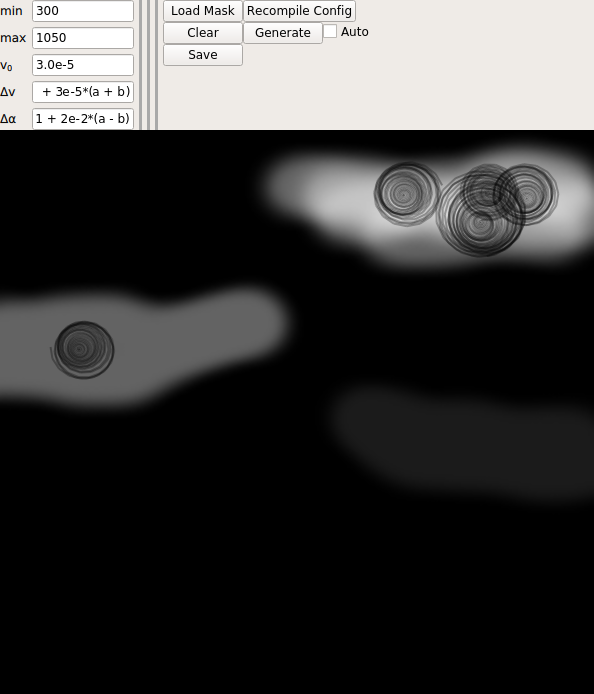
\includegraphics[width=11cm]{images/app.png}
  \caption{Vzhľad Aplikácie}
\end{figure}

\FloatBarrier

\section{Parametrizácia tvaru krivky}

Tvar krivky sa generuje následujúcim spôsobom. Vygeneruje sa náhodná dĺžka $l$
krivky v rozmedzí parametrov \emph{min} a \emph{max}. Potom sa vygeneruje $l$
zoznamov hodnôt motorov $ms$. $ms$ sa skladá z $n$ náhodných hodnôt od -1 po 1,
kde $n$ je počet premenných vo výrazoch $\Delta v$ a $\Delta \alpha$. Následne
sa pre každý zoznam hodnôt motorov $ms$ vypočítajú hodnoty $\Delta v$ a $\Delta
\alpha$ (zrýchlenie štetca a zmena uhla štetca) podľa príslušných výrazov.
Diskrétnou integráciou sa vypočítajú hodnoty

\begin{equation}
  v_i = v_0 + \sum{\Delta v_j}_{j = 1 .. i}
\end{equation}.

Následne sa vygeneruje náhodná počiatočná pozícia a uhol natočenia štetca a opäť
pomocou diskrétneho integrálu sa z hodnôt rýchlostí a zmien uhlov určia náhodne
pozície v časoch $1 .. l$.

Výrazy $\Delta v$ a $\Delta \alpha$ musia byť platné výrazy v jazyku Haskell,
ich typ musí byť $Double$. Ak toto nie je splnené, do terminálu sa vypíšu
chybové hlášky. \emph{min} a \emph{max} musia byť celé čísla, $v_0$ musí byť
číslo typu $Double$.

\section{Parametrizácia štýlu krivky}

Parametrizácia tvaru krivky je prívetivá pre užívateľa, ale je obmedzujúca.
Parametrizácia štýlu krivky je naopak dosť voľná, ale je písaná v jazyku
Haskell. Uživateľ neznalý tohto jazyka by však mal byť schopný vybrať si
spomedzi štyroch preddefinovaných štýlov a prenastaviť aspoň farbu a hrúbku
štetca. Po spustení aplikácie z terminálu sa doň vypíše cesta ku konfiguračnému
súboru. V ňom môže uživateľ vykonať zmeny a tlačidlom \emph{Recompile Config} ho
môže prenačítať v aplikácii.

\section{Parametrizácia uživateľského rozhrania}

Ak uživateľovi nevyhovuje vzhľad aplikácie, môže si ju nastaviť v súbore na
ceste rovnakej, ako cesta ku konfiguračnému súboru, ale namiesto
\texttt{cfg/Config.hs} je \texttt{qml/Main.qml}.

\section{Galéria výstupov}

\FloatBarrier

\begin{figure}[!h]
  \centering
  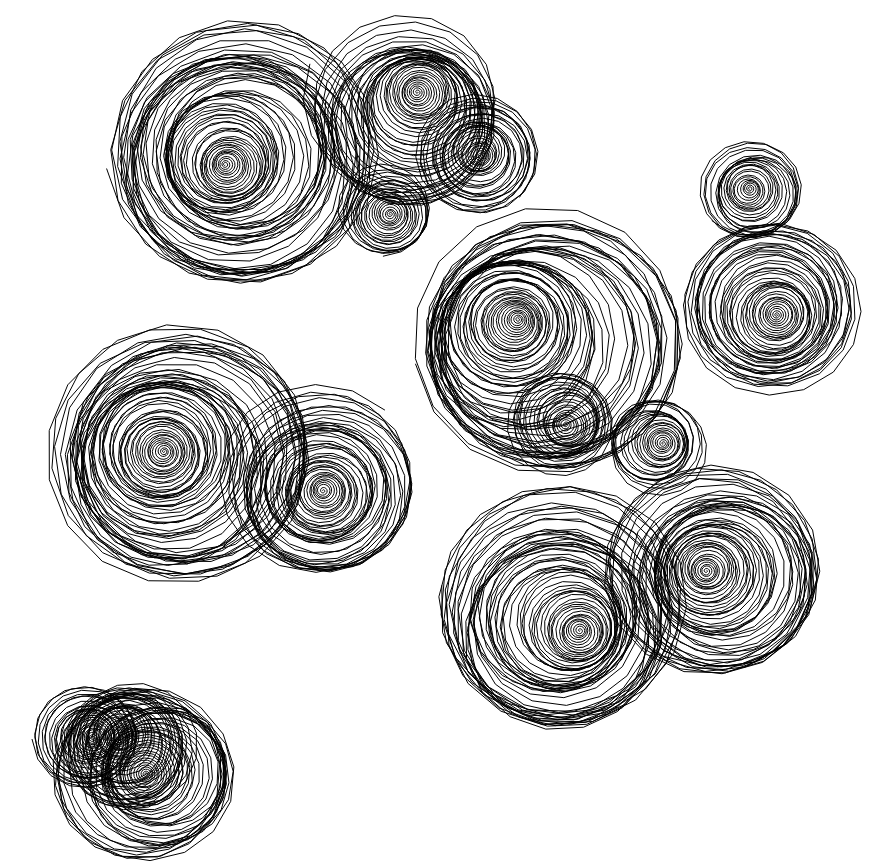
\includegraphics[width=10cm]{images/snails.png}
  \caption{Slimáky}
\end{figure}

\begin{figure}[!h]
  \centering
  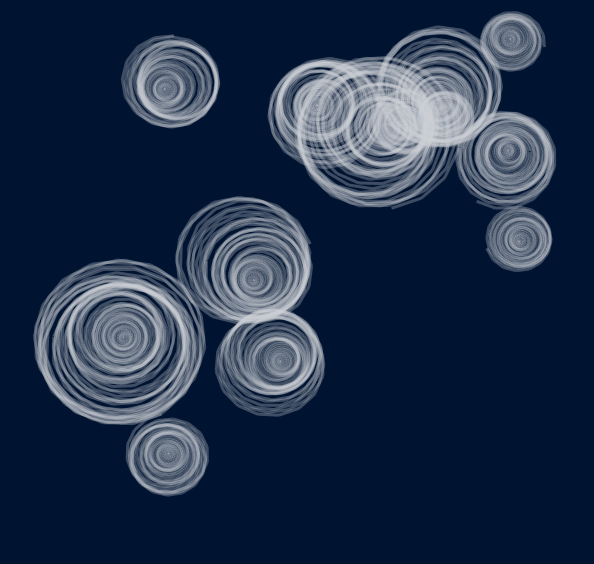
\includegraphics[width=10cm]{images/bubbles.png}
  \caption{Bubliny}
\end{figure}

\begin{figure}[!h]
  \centering
  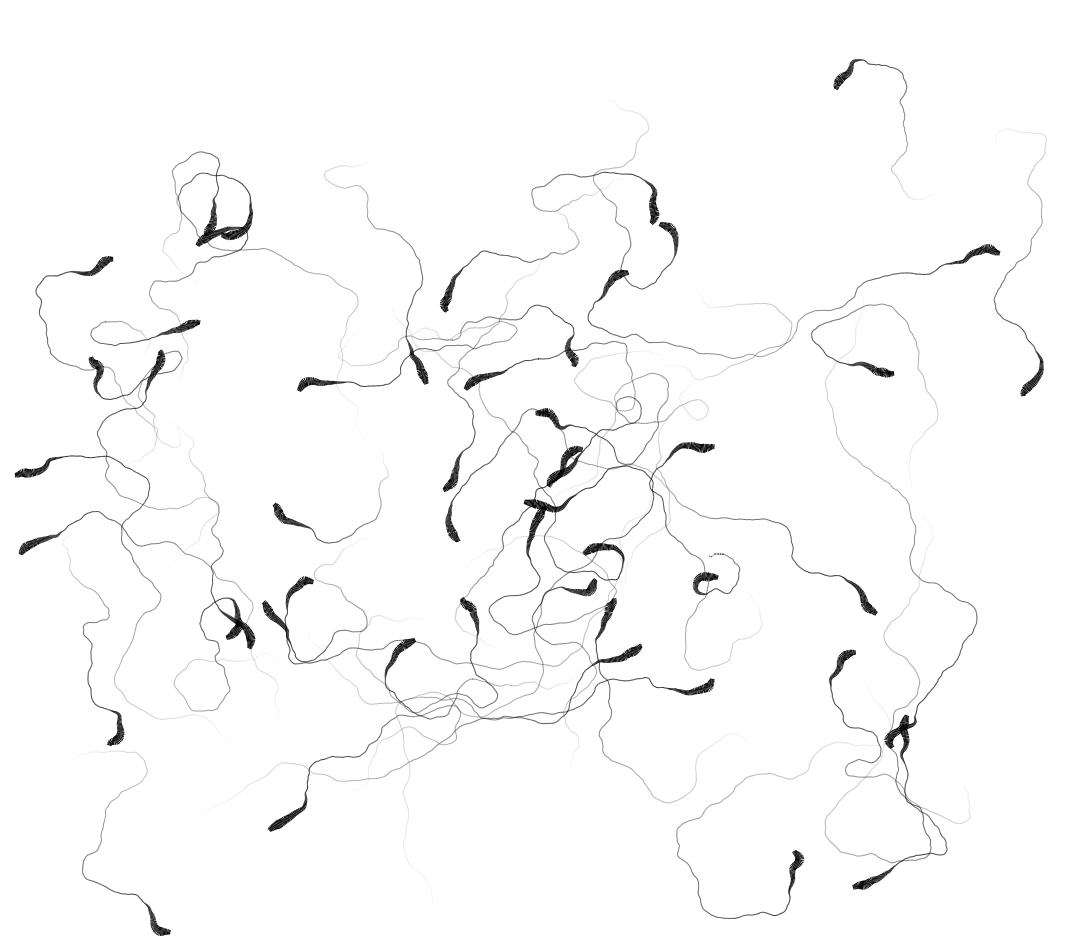
\includegraphics[width=10cm]{images/tadpoles.png}
  \caption{Žubrienky}
\end{figure}

\begin{figure}[!h]
  \centering
  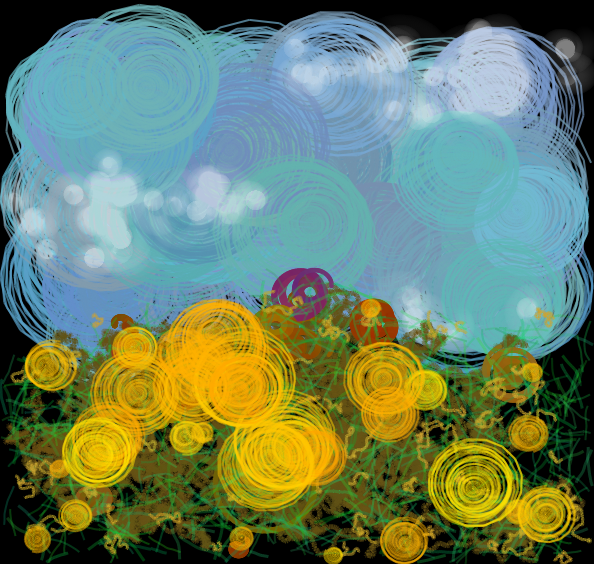
\includegraphics[width=10cm]{images/hill.png}
  \caption{Jar}
\end{figure}

\FloatBarrier


\section{Implementácia}

Aplikácia je naprogramovaná v jazyku Haskell. Pre dynamickú kompiláciu výrazov a
konfiguračného súboru je použitá knižnica \emph{hint}. Grafické uživateľské
rozhranie je vytvorené pomocou deklaratívneho jazyka QML (z knižnice Qt5) a je
prepojené s jadrom aplikácie pomocou knižnice \emph{hsqml}. Logika grafického
uživateľského rozhrania je implementovaná taktiež deklaratívne, pomocou
teoretického modelu \emph{FRP (Functional Reactive Programming)},
implementovaného knižnicou \emph{Yampa}.

\section{Kompilácia}

Aplikácia je závislá na knižnici \emph{Qt5}. Pre jej jednoduchú kompiláciu je
potrebné mať nainštalovaný program \emph{cabal-install}, ktorý býva štandardnou
súčasťou Linuxových distribúcií. Na Windowse je tento program obsiahnutý v
balíku \emph{Haskell Platform}. Vojdite do adresára projektu a v príkazovom
riadku vykonajte následovné:

\texttt{cabal sandbox init}

\texttt{cabal install}

Aplikácia je takto nainštalovaná v separovanom prostredí, tzv. \emph{sandbox},
aby sme sa vyhli konfliktom s prípadnými inými knižnicami GHC nainštalovanými v
systéme, a jej spustiteľný program sa v prípade Linuxu nachádza na ceste
\texttt{.cabal-sandbox/bin/digital\_impro}.

Na platforme Windows som to netestoval, ale nevidím dôvod, prečo by to nemalo
fungovať, v prípade, že sa ale nechcete stretnúť so žiadnymi problémami a máte k
dispozícii Linux, použite radšej Linux.

\section{Plány do budúcna}

Pipeline generovania krivky je pevne daný a to mi príde príliš obmedzujúce.
Tento pipeline by mohol byť taktiež konfigurovateľný v jazyku Haskell. Potom by
však mali byť konfigurovateľné aj widgety, ktoré nastavujú jeho parametre. Takým
istým spôsobom by sa mohli generovať aj widgety ovládajúce štýl krivky. Vznikla
by z toho takto pekná minimalistická a vysoko konfigurovateľná aplikácia pre
tvorenie umenia. Dalo by sa nakonfigurovať aj kreslenie myšou, namiesto
náhodného generovania obrazcov.

\end{document}
